\documentclass{beamer}
%\usepackage{xcolor}

\usepackage{tikz}
\usepackage{tikzducks,tikzlings}
%\usepackage{../sheep-tikzling/tikzlings-sheep}
\usetikzlibrary{shapes.callouts}

\setbeamertemplate{background}
{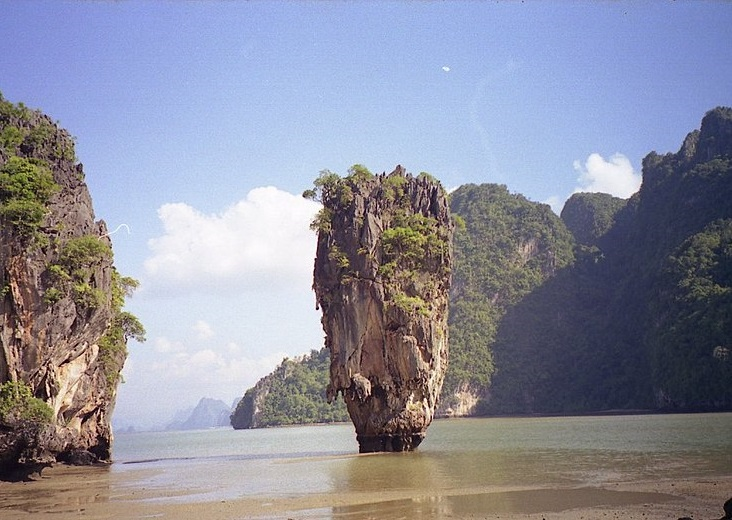
\includegraphics[width=\paperwidth,height=\paperheight]{James_Bond_Island_-_panoramio.jpg}}

\setbeamertemplate{navigation symbols}{}

\begin{document}

\begin{frame}
\begin{tikzpicture}[remember picture, overlay]
\begin{scope}[yshift=0.75cm,xshift = 5.5cm]
	\sheep[%cocktail,
    body=brown!50!darkgray!97!yellow!20!white,
    scale=0.8,
		bubblecolour=gray!30!white];
   \node at (0.0,0.6) {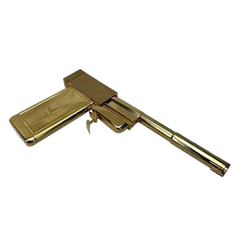
\includegraphics[width=1cm]{colt}};
   \node at (0.0,1.3) {
\includegraphics[width=20pt]{sunglasses.png}};
\end{scope}
\begin{scope}[yshift=-5.25cm,xshift=-50+0.54*\thepage,yscale=0.7]
  \penguin
  \fill[black!70!white] (0.1,1.94) ellipse[x radius=0.48, y radius=0.1, rotate=-15];
  \fill[black!70!white] (0.46,1.9) arc [radius=0.37, start angle=-15, end angle=165];
  \node[rotate=20] at (-0.6,0.7) {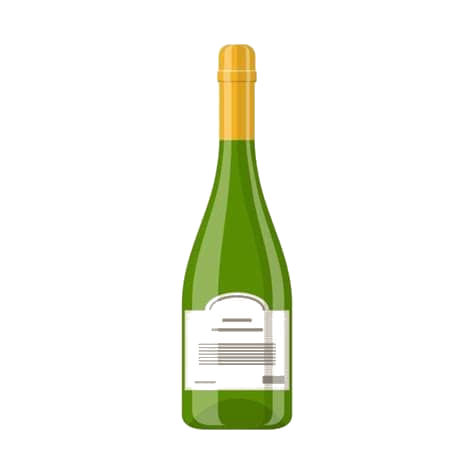
\includegraphics[width=1cm]{bottle}};  
\end{scope}
\pause[500]
\end{tikzpicture}
\end{frame}

\foreach \x in {0,...,200}{
\begin{frame}
\begin{tikzpicture}[remember picture, overlay]
\begin{scope}[yshift=0.75cm,xshift = 5.5cm]
	\sheep[%cocktail,
    body=brown!50!darkgray!97!yellow!20!white,
    scale=0.8,
		bubblecolour=gray!30!white];
   \node[ellipse callout,fill=white!80!gray,callout absolute pointer={(0.8,1.4)},text width=3cm, align=center] at (2.8,2) {My name is Baaa, James Baaa!}; 
   \node at (0.0,0.6) {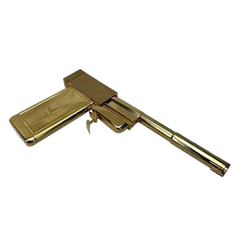
\includegraphics[width=1cm]{colt}};
   \node at (0.0,1.3) {
\includegraphics[width=20pt]{sunglasses.png}};
\end{scope}
\begin{scope}[yshift=-5.25cm,xshift=220,yscale=0.7]
  \penguin
  \fill[black!70!white] (0.1,1.94) ellipse[x radius=0.48, y radius=0.1, rotate=-15];
  \fill[black!70!white] (0.46,1.9) arc [radius=0.37, start angle=-15, end angle=165];
  \node[rotate=20] at (-0.6,0.7) {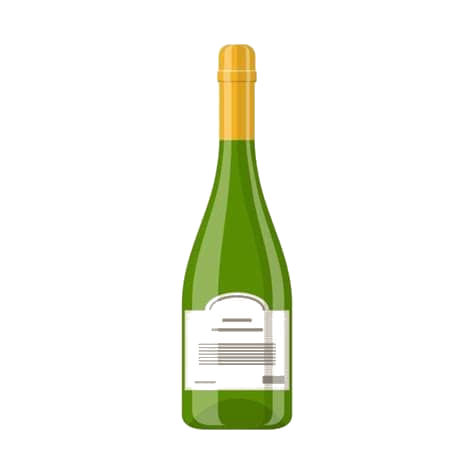
\includegraphics[width=1cm]{bottle}};  
\end{scope}
\end{tikzpicture}
\end{frame}
}

\end{document}